
\documentclass[draft,linenumbers]{agujournal2019}

\usepackage{url} 
\usepackage{lineno}
% \usepackage[inline]{trackchanges} 
\usepackage{soul}
\usepackage{natbib}
\usepackage{float}

%\draftfalse

\journalname{JGR Oceans}

%%%%%%%%%%%%%%%%%%%%%%%%%%%%%%%%%%%

%% MACROS
\newcommand{\MKE}{\overline{\textrm{KE}}}
\newcommand{\mKE}{\textrm{MKE}}
\newcommand{\KE}{\textrm{KE}}
\newcommand{\MEKE}{\overline{\textrm{EKE}}}
\newcommand{\EKE}{\textrm{EKE}}
\newcommand{\MCEKE}{\overline{\textrm{CEKE}}}
\newcommand{\CEKE}{\textrm{CEKE}}
\newcommand{\MnCEKE}{\overline{\textrm{nCEKE}}}
\newcommand{\nCEKE}{\textrm{nCEKE}}
\newcommand{\cEddy}{\textrm{cEddy}}

\begin{document}
\title{Climatology, seasonality and trends of oceanic coherent eddies}

\authors{Josu\'e Mart\'inez-Moreno\affil{1}, Andrew McC. Hogg\affil{1}, and Matthew H. England\affil{2}}
\affiliation{1}{Research School of Earth Science and ARC Center of Excellence for Climate Extremes, Australian National University, Canberra, Australia}
\affiliation{2}{Climate Change Research Centre (CCRC), UNSW Australia, Sydney NSW, Australia}

\correspondingauthor{Josu\'e Mart\'inez-Moreno}{josue.martinezmoreno@anu.edu.au}

\begin{keypoints}
	\item Kinetic energy of coherent eddies 
	contain around 50\% of the 
	surface ocean kinetic energy budget.
	\item Seasonal cycle of the number of coherent eddies and 
	coherent eddy amplitude reveal a 3-6 month lag to wind forcing
	\item Inverse cascade sets up the seasonal lag of the number and amplitude of coherent eddies.
	\item The coherent eddy amplitude has increase at 
	a rate of 3 cm per decade since 1993.
\end{keypoints}


\begin{abstract}
	
	Ocean eddies influence regional and global climate through mixing and transport of heat and properties. 
	One of the most recognizable and ubiquitous feature of oceanic eddies are vortices with spatial scales of tens to hundreds of kilometers, frequently referred as ``mesoscale eddies" or ``coherent eddies". 
	Coherent eddies are known to transport properties across the ocean and to locally affect near-surface wind, cloud properties and rainfall patterns. Although coherent eddies are ubiquitous, yet their climatology, seasonality and long-term temporal evolution remains poorly understood. 
	Thus, we examine the kinetic energy contained by coherent eddies and we present the annual and long-term changes of automatically identified coherent eddies from satellite observations from 1993 to 2018. 
	Around 50\% of the kinetic energy contained by ocean eddies corresponds to coherent eddies. 
	Additionally, a strong hemispherical seasonal cycle is observed, with a 3--6 months lag between the wind forcing and the response of the coherent eddy field. 
	Furthermore, the seasonality of the number of coherent eddies and their amplitude reveals that the number of coherent eddies responds faster to the forcing ($\sim$3 months), then the coherent eddy amplitude (which is lagged by $\sim$6 months).  
	%There are regions that show a pronounced influence of coherent eddies, notably, the East Indian Ocean, the East Tropical Pacific Ocean, and the South Atlantic Ocean. 
	%In these locations, a strong seasonal cycle and interannual variability can be observed in both satellite and numerical models. Although, there is agreement between these products on the seasonality of the number of eddies, the seasonality of the coherent eddy amplitude between these products show some inconsistencies. 
	%Long-term trends of the coherent eddy amplitude from satellite observations and the state of the art model show significant increases in the eddy amplitude of $\sim$3cm per decade in large portions of the ocean, while the number of coherent eddies remains constant. 
	Our analysis highlights the relative importance of the coherent eddy field in the ocean kinetic energy budget, implies a strong response of the eddy number and eddy amplitude to forcing at different time-scales, and showcases the seasonality, and multidecadal trends of coherent eddy properties. 

	\noindent\textbf{Plain language summary}
	
\end{abstract}	

\section{Introduction}

Mesoscale ocean variability with spatial scales of tens to hundreds of kilometers is comprised of processes such as vortices, waves, and jets \citep{Ferrari_energy_2009, Fu_Eddy_2010}. 
These mesoscale processes are highly energetic, and they play a crucial role in the transport of heat, salt, momentum, and other tracers through the ocean \citep{Wunsch_energetics_2004, Wyrtki_Eddy_1976, Gill_Energy_1974}. Possibly, the most recognizable and abundant process observed from satellites is mesoscale vortices. Although mesoscale vortices are commonly referred to in literature as ``mesoscale eddies", this term is also often used to describe the total mesoscale ocean variability (the time-varying component of the mesoscale flow), thus, here we will refer to mesoscale vortices as \emph{coherent eddies}. 


Coherent eddies are quasi-circular currents. According to their rotational direction, the sea surface height anomaly within a coherent eddy can have a negative or positive sea surface height anomaly (cold-core and warm-core coherent eddies, respectively). 
This characteristic sea surface height signature of coherent eddies has been utilized to automatically identify and track coherent eddies from satellite altimetry \citep{Cui_eddy_identification_2020,Martinez_TKE_2019, Ashkezari_eddies_2016, Faghmous_A_2015,Chelton_Global_2007}. 
Automated identification algorithms of coherent eddies have shown their ubiquity in the oceans, with a predominant influence at hotpots of eddy activity such as boundary currents and the Antarctic Circumpolar Current. In these regions, \citet{Chelton_The_2011} estimated that coherent eddies contribute around 40--50\% of the mesoscale kinetic energy \citep{Chelton_The_2011} and thus a significant fraction of the total kinetic energy \citep{Ferrari_energy_2009}. Although this unique estimate showcases the importance of the mesoscale coherent eddy field, the energy contained by coherent eddies was estimated by extracting the geostrophic velocities within the detected coherent eddies, thus it is possible it may contain energy from other processes. Coherent eddies are not only abundant and may have a large proportion of the surface kinetic energy budget, but they are also essential to ocean dynamics as concluded by many previous studies \citep{Patel_SO_eddies_2020,Schubert_submesoscale_2019,Pilo_eddy_2015,Frenger_Southern_2015,Frenger_Imprint_2013,BeronVera_Agulhas_2013,Siegel_Bio_2011,Hogg_Interdecadal_2006}.


There is broad consensus that mesoscale eddy kinetic energy has a pronounced seasonal variability \citep{Uchida_Seasonality_2017,Kang_On_2017,Qiu_seasonal_2004, Qiu_seasonal_1999}. 
Several hypotheses have been proposed to explain this seasonality including: seasonal variations of atmospheric forcing \citep{Sasaki_seasonal_2014}, seasonality of the mixed layer depth \citep{Qiu_seasonal_2014,Callies_season_2015}, seasonality of the intensity of barotropic instability \citep{Qiu_seasonal_2004}, the variability of the baroclinic instability due to the seasonality of the vertical shear \citep{Qiu_seasonal_1999}, and a seasonal lag of the inverse energy cascade (energy is transported between scales from small to large; \citealp{Arbic_cascade_2013}) in combination with the presence of a front in the mixed layer, which can lead to a seasonal cycle of the baroclinic instability \citep{Qiu_seasonal_2014}. On one hand, processes such as barotropic and baroclinic instabilities control the seasonality of coherent eddies in the ocean. 
On the other hand, recent studies using observations and eddy-permitting climate models suggest several long-term adjustments of the global ocean capable of long-term changes in the coherent eddy field. 
Such readjustments include a multidecadal increase in the ocean stratification resulted from temperature and salinity changes \citep{Li_stratification_2020}, a horizontal readjusment of the sea surface temperature gradients \citep{Ruela_SST_trends_2020,Bouali_SST_grad_trends_2017,Cane_SST_trends_1997}, and an intensification of the kinetic energy, eddy kinetic energy, and mesoscale eddy kinetic energy over the last 3 decades as a consequence of an increase in wind forcing \citep{Hu_acceleration_2020,Wunsch_speeding_2020,Martinez_Kinetic_2021}. All these seasonal factors and long-term readjustments directly influence the annual and decadal response of the coherent eddy field, however, the seasonality of the coherent component of the eddy kinetic energy, as well as the seasonal cycle and trends of the coherent eddy statistics remain unknown.

Here we present a new global climatology of the coherent eddy kinetic energy by reconstructing the coherent eddy signature from satellite observations. Our climatology documents the seasonal cycle of the coherent eddy kinetic energy, and seasonal cycle and long-term trends of the coherent eddy properties over the satellite record. 
Moreover, we conduct more detail analysis in regions where coherent eddies dominate the eddy kinetic energy field. 
This paper is structured as follows:  the data sources and methodology are described in section \ref{sec:Methods}.
Then, we present the climatology, energy ratios, and global seasonality of the coherent eddy kinetic energy in subsection \ref{subsec:CEKE_climatology}. 
Subsection \ref{subsec:CE_stats} presents the global climatology and seasonality of coherent eddy properties, followed by the seasonal cycle and coherent eddy property time-series in regions dominated by coherent eddies (subsection \ref{sec:CE_regional_stats}). 
We then focus our attention on the long-term changes of the coherent eddy properties (section \ref{sec:CE_trends}). 
Finally, section \ref{sec:Conclusions} summarizes the main results and discusses the implications of this study.

\section{Methods}
\label{sec:Methods}
	We use daily sea surface height (SSH) data made available by the Copernicus Marine Environment Monitoring Service in near real time \citep{CMEMS_aviso_2017}. 
	This gridded product contains the sea surface height and geostrophic velocities with daily 0.25$^\circ$ resolution from January 1993 to 2019.
	The daily geostrophic velocities allowed us to compute the kinetic energy ($\KE$) and eddy kinetic energy ($\EKE$) over the satellite record. The main source of $\EKE$ is the time-varying wind \citep{Ferrari_energy_2009}, thus we computed the seasonal cycle of the wind magnitude from the JRA55 reanalysis \citep{JMA_JRA55_2013} using wind velocities at 10m above the ocean's surface. 

	Over the same record, coherent eddy statistics from \citet{Martinez_TKE_2019}, hereafter M-M, are analyzed and compared to those released by \citet{Chelton_mesoscale_2013}, both datasets are gridded in a 1$^\circ$ resolution. 
	Although both datasets are produced via automated eddy identification algorithms using closed contours of SSH, these datasets have important differences in the criteria they use to identify and record coherent eddies statistics. 
	The major difference include; (i) M-M's algorithm requires an adjustment between a 2D Gaussian and the SSH anomaly (SSHa) surface within the identify closed contour, while Chelton's only uses the outer-most closed contour of SSH; (ii) M-M's dataset reports the maximum SSHa within the identified coherent eddy, while Chelton's algorithm reports the maximum SSH value minus the discrete level in which the coherent eddy was identified; M-M's dataset includes all detected coherent eddies, while Chelton's dataset excludes (iii) coherent eddies with lifetimes shorter that four weeks and (iv) coherent eddy amplitudes smaller than 1cm. Moreover, M-M's algorithm allows the reconstruction of the coherent eddy field under the assumption that coherent eddies have a 2D Gaussian imprint in the sea surface height. These Gaussian anomalies then allow us to estimate the coherent geostrophic eddy velocities and thus the kinetic energy contained only by coherent eddies.

	\subsection{Kinetic Energy decomposition}

	Kinetic energy is commonly divided into the mean and time-varying components through a Reynolds decomposition. At a given time, the velocity field $\mathbf{u} = (u,v)$ is split into the time mean ($\mathbf{\overline{u}}$) and time varying components ($\mathbf{u'}$). Moreover, M-M proposed to further decompose the eddy kinetic energy into the energy contained by coherent features ($\mathbf{u'_e}$) and non-coherent features ($\mathbf{u'_n}$). Therefore the KE equation can be written as:
	
	\begin{equation}
		\mathrm{KE} = \underbrace{\overline{u}^2 + \overline{v}^2}_{\mKE} + 
		\underbrace{\underbrace{{u'}_e^2+{v'}_e^2}_{\CEKE}  + \underbrace{{u'}_n^2+{v'}_n^2}_{\nCEKE} + \mathcal{O}_c^2 }_{\EKE} + \mathcal{O}^2
	\end{equation}

	Due to the properties of this decomposition, the second order term $\mathcal{O}^2$ is zero when averaged over the same period as $\mathbf{\overline{u}}$. However, $\mathcal{O}_c^2$ is negligible when averaged over time and space. More information about the decomposition of the field into coherent features and non-coherent features is explained by \citet{Martinez_TKE_2019}. A global snapshot of each component of kinetic energy decomposition is shown in Figure \ref{fig:eddy_snapshot}, where the $\KE$ and $\EKE$ are comprised of rings and filaments. As expected, the decomposition of $\EKE$ into $\CEKE$ and $\nCEKE$ components exhibit only ring-like signatures expected of coherent eddies, while the non-coherent component shows filaments and some unidentified coherent eddies.

	\begin{figure}[t]
	    \centering
	    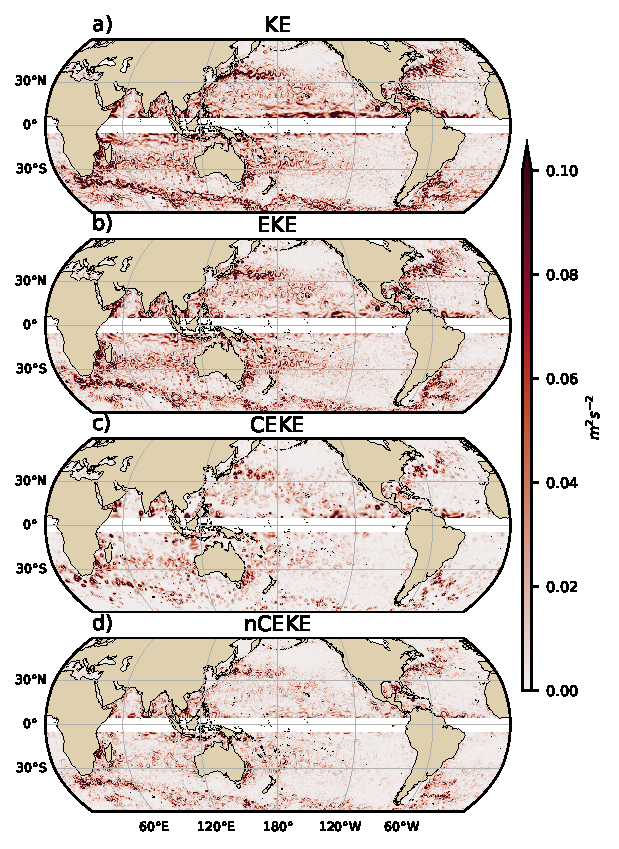
\includegraphics[width=95mm]{figures/snapshot_ke_maps_satellite_large.pdf}
	    \caption{Snapshot of surface kinetic energy ($\MKE$), surface eddy kinetic energy ($\MEKE$), surface coherent eddy kinetic energy ($\MCEKE$), and surface non-coherent eddy kinetic energy ($\MnCEKE$) for the 1st of January 2017.}
	    \label{fig:eddy_snapshot}
	\end{figure}

	\subsection{Eddy statistics}

	The eddy statistics used in this study include the eddy count ($\mathrm{cEddy}_{n}$) defined as the number of eddies per grid cell, and the mean eddy amplitude defined as the mean amplitude of the coherent eddies within the cell ($\mathrm{cEddy}_{amp}$), The latter metric can be separated into positive ($\mathrm{cEddy}_{amp}^{+}$) and negative ($\mathrm{cEddy}_{amp}^{-}$) coherent eddy amplitudes, defined as the mean amplitude of warm core and cold core coherent eddies, respectively, within the cell. 
	The absolute eddy amplitude ($|\mathrm{cEddy}_{amp}|$) is then defined as:
	\begin{equation}
	|\mathrm{cEddy}_{amp}| = \frac{1}{2} \left(\mathrm{cEddy}_{amp}^{+} -  \mathrm{cEddy}_{amp}^{-} \right)
	\end{equation}
	Note that the $\mathrm{cEddy}_{amp}^{+}$ and $\mathrm{cEddy}_{amp}^{-}$ are sign definite, thus the difference will always be positive, mean $\mathrm{cEddy}_{amp}$ can be negative or positive noting the dominant polarity of coherent eddies in the region. We analyze the climatology, seasonal cycles and trends of the eddy statistics between 1993 and 2019. We exclude the equatorial region (10$^\circ$S - 10$^\circ$N) and poleward of 60$^\circ$. Note that the climatology of $\mathrm{cEddy}_{n}$ is computed by adding all the identified eddies over the record, while all other climatological statistics are computed as the time-average over the record.  Seasonal climatologies are calculated for the monthly average of each coherent eddy statistic, while hemispherical time-series are filtered with a running average of 90 days. Trends of $\mathrm{cEddy}_{n}$ and $|\mathrm{cEddy}_{amp}|$ are calculated by coarsening the dataset to a 5$^\circ$ grid, and then linear trends are computed for each grid point, the statistical significance is assessed by a modified Mann-Kendall test \citep{Sheng_MK_2004}. Time averages are denoted by $\overline{\phantom{X}}$, while area averages are shown by $\left< \phantom{X}\right>$.

	\section{Global Coherent Eddy Energetics}
	\label{subsec:CEKE_climatology}

	% \textbf{Figure 2}
	% \begin{itemize}
	% 	\item All KE components have large energy contents in the boundary currents and antarctic circumpolar current. 
	% 	\item In many cases is the same, but there actually some differences There are several regions where the coherent component is larger than the non-coherent, we will investigate these in more detail in section XX.
	% \end{itemize}

	The climatology geostrophic components of the kinetic energy decomposition estimated from sea surface height are shown in Figure \ref{fig:eddy_climatology}. These maps show that many regions of the global ocean are highly energetic in mean KE ($\MKE$), mean EKE ($\MEKE$), mean coherent eddy kinetic energy ($\MCEKE$) and mean non-coherent eddy kinetic energy ($\MnCEKE$). The spatial pattern highlights well known regions of the ocean, where mesoscale processes are abundant, such is the case of western boundary currents, the Antarctic Circumpolar Current and regions within the ocean gyres. Remarkably, the spatial distribution of the energy contained by the reconstructed mesoscale coherent eddies and non-coherent components are similar (Figures \ref{fig:eddy_climatology}c,d), which can be thought as regions where mesoscale activity is intense, however, there are some regions where coherent eddies dominate over non-coherent and vice-versa. Overall, this decomposition suggest that boundary currents and other energetic regions, in particularly, eddy-rich regions in the ocean contain both coherent and non-coherent components of the kinetic energy.

	\begin{figure}[t]
	    \centering
	    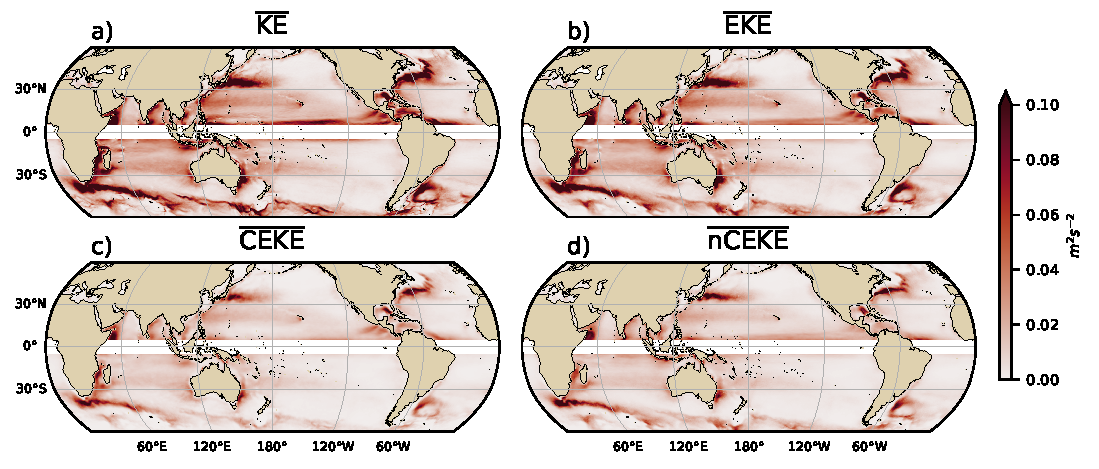
\includegraphics[width=1\textwidth]{figures/mean_ke_maps_satellite.pdf}
	    \caption{Climatology of surface kinetic energy ($\MKE$), surface eddy kinetic energy ($\MEKE$), surface coherent eddy kinetic energy ($\MCEKE$), and surface non-coherent eddy kinetic energy ($\MnCEKE$) between 1993-2018.}
	    \label{fig:eddy_climatology}
	\end{figure}

	% \textbf{Figure 3}
	% \begin{itemize}
		% \item $\MEKE$ is responsible of almost all the $\MKE$ across the ocean, except for regions with persistent currents over time, such as the mean boundary current locations, equatorial pacific currents and regions in the Antarctic Circumpolar current, where the EKE explains around 40\% of the $\MKE$
		% \item This estimate is consistent with that of Chelton.
		% \item $\MEKE$ Explains $~80\%$ of $\MKE$, while $\MCEKE$ is $~45\%$ of $\MEKE$ and $\MnCEKE$  is $~60\%$ of $\MEKE$ 
		% \item $\MCEKE$ is large equatorwards from the Kuroshio current and Agulhas current.
		% \item Areas with the largest coherent contribution are located in the South of Australia $\MCEKE$ and South Atlantic
		% \item 
		% \item $\MnCEKE$ has a large amount of energy at high latitudes, this could be a consequence of the satellites not resolving the mesoscale coherent eddies. 
	% 	\item Global averages of the ratios show $\MEKE$ explains around 78\% of the ocean $\MKE$ field, while coherent eddies and non coherent eddy features contain 49\% and 59\% percent. Note this values don't add to 1 as there are cross terms that contain around XX\% of the total energy.
	% \end{itemize}


	\begin{figure}
	    \centering
	    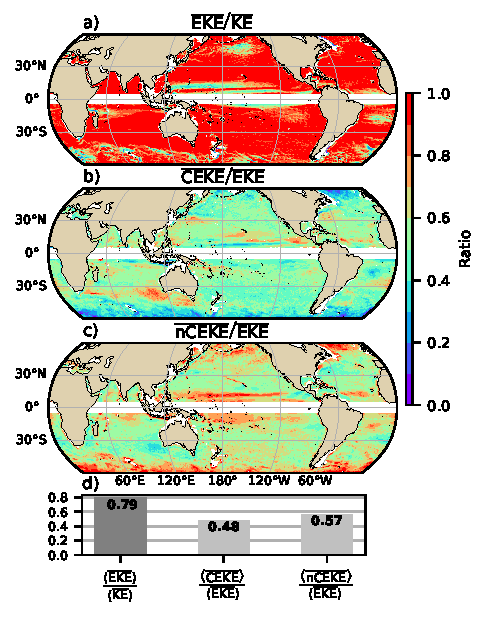
\includegraphics[width=1\textwidth]{figures/eke_ratio_map_easy.pdf}
	    \caption{Ratios of the kinetic energy components. a) Map of the proportion of mean eddy kinetic energy ($\EKE$) versus mean kinetic energy ($\MKE$);
		b) Map of the percentage of mean coherent eddy kinetic energy ($\MCEKE$) versus mean eddy kinetic energy ($\MEKE$);
		c) Map of the percentage of mean non-coherent eddy kinetic energy ($\MnCEKE$) versus mean eddy kinetic energy ($\MEKE$);
		d) Global area averaged percentage of mean eddy kinetic energy ($\left<\MEKE\right>$) versus the global mean kinetic energy ($\left<\MKE\right>$), area averaged percentage of mean coherent eddy kinetic energy ($\left<\MCEKE\right>$) and mean non coherent eddy kinetic energy ($\left<\MnCEKE\right>$) versus global mean eddy kinetic energy ($\left<\MEKE\right>$). Regions where the depth of the ocean is shallower than 1000m are removed from the ratio estimation.
		}
	    \label{fig:eddy_ratio}
	\end{figure}

	Eddy kinetic energy is known to be more than an order of magnitude greater than $\mKE$ \citep{Gill_Energy_1974}, this is clearly shown in Figure \ref{fig:eddy_ratio}a, where the ratio of $\MEKE$ is responsible of almost all the $\MKE$ across the ocean, except for regions with persistent currents over time. 
	Such regions are located in the mean boundary current locations, the equatorial pacific currents and regions in the Antarctic Circumpolar current, where the EKE explains around 40\% of the $\MKE$. 
	As estimated by a previous study by \citet{Chelton_The_2011}, the $\EKE$ within coherent eddies with lifetimes greater than 4 weeks contain between 40 to 60 percent of the $\MEKE$. 
	Our result from reconstructing the coherent eddy signature (Figure \ref{fig:eddy_ratio}b) further corroborates that the coherent component ($\MCEKE$) has around 50\% of the $\MKE$ (Figure \ref{fig:eddy_ratio}d). 
	Furthermore, global averages of the ratios show $\MEKE$ explains approximately 78\% of the ocean $\MKE$ field, while non coherent eddy features contain 48\% and 57\% percent. 
	Note the globally averaged coherent and non coherent components do not add to 100\% as the cross terms ($\mathcal{O}_c^2$) are different to zero. 
	This is likely to errors in the coherent eddy reconstruction. 
	The spatial pattern reveals a dominance of the $\MCEKE$ equatorward from the boundary currents and areas with large coherent eddy contributions of around 90\% of the region's eddy kinetic energy, for example, south of Australia, Tehuantepec Gulf and South Atlantic. 
	An evident signal is an reduction of the energy contained by coherent eddies at high latitudes and an increase in the energy explained by non-coherent eddies, this could be a consequence of the incapability of the 0.25$^\circ$ satellite resolution ($\sim$ 13 km at 60$^\circ$) to fully resolve coherent eddies with scales smaller than $\sim$10 km (first baroclinic Rossby radius at 60$^\circ$)



	\subsubsection{Seasonality}

	% \textbf{Figure 4}
	% \begin{itemize}
		% \item The hemisphere seasonality show the  $\EKE$ and $\CEKE$ peak in summer.
		% \item Response of the $\EKE$ and $\CEKE$ show a seasonal lag of $\sim$6 months to the forcing of the Winds. Make sure to note the maximum over the hemisphere, locally, the winds may peak in different months. 
		% \item The coherent eddy field show a large interannual variability.
		% \item In the Southern Ocean we observe a concentric growth as time passes, which support the increasing trends in the Southern Ocean observed by \citep{Hogg_Recent_2015,Martinez_TKE_2019,Martinez_Kinetic_2021}
		% \item Point that in the northern hemisphere in winter the CEKE appears to be decreasing.
	% \end{itemize}

	In accordance with the previously observed $\EKE$ seasonal cycle, we investigate seasonal cycle of the $\EKE$ and $\CEKE$ for the northern hemisphere (NH; 10$^\circ$N - 60$^\circ$N) and Southern Hemisphere (SH; 60$^\circ$S - 10$^\circ$S). 
	In both hemispheres (Figure \ref{fig:eddy_energy_polar}), the $\EKE$ and $\CEKE$ peak during the hemispherical summer. In the northern hemisphere, the largest $\EKE$ and $\CEKE$ occurs $\sim$6 months after the maximum winds (Figure \ref{fig:eddy_energy_polar}c and d), while the Southern ocean seems to respond within $\sim$4 months (Figure \ref{fig:eddy_energy_polar}g, and h). This seasonal lag and maximum is consistent with a time-lag of the inverse cascade \citep{Sasaki_seasonal_2014, Qiu_seasonal_2014} where winter has the highest energy at the smallest scales (non-solvable with satellite observations), spring and autumn have the highest and lowest energy in scales of 50-100 km, and summertime has the highest energy at the largest scales ($>$ 100 km; \citealt{Uchida_Seasonality_2017}), thus the maximum of $\EKE$ and $\CEKE$ located during summertime suggest eddies and coherent eddies have scales larger than 100 km.

	The cyclic plots in Figure \ref{fig:eddy_energy_polar} shows the temporal evolution of $\EKE$ and $\CEKE$. 
	Note that high frequency variability can be observed in the $\CEKE$ field with temporal scales of a few months, this could be attributed local dynamics averaged over the hemisphere, as well as errors within the coherent eddy identification. 
	% This signature will be further explored in section \ref{sec:CE_regional_stats}.
	Additionally, cyclic plots highlight long-term temporal changes over the record; (i) northern hemisphere winters show a decrease in the $\CEKE$ field and (ii) the Southern hemisphere show concentric growth over time in $\EKE$ and $\CEKE$, which support the increasing trends in the Southern Ocean observed by \citep{Hogg_Recent_2015,Martinez_TKE_2019,Martinez_Kinetic_2021}. 

	\begin{figure}
	    \centering
	    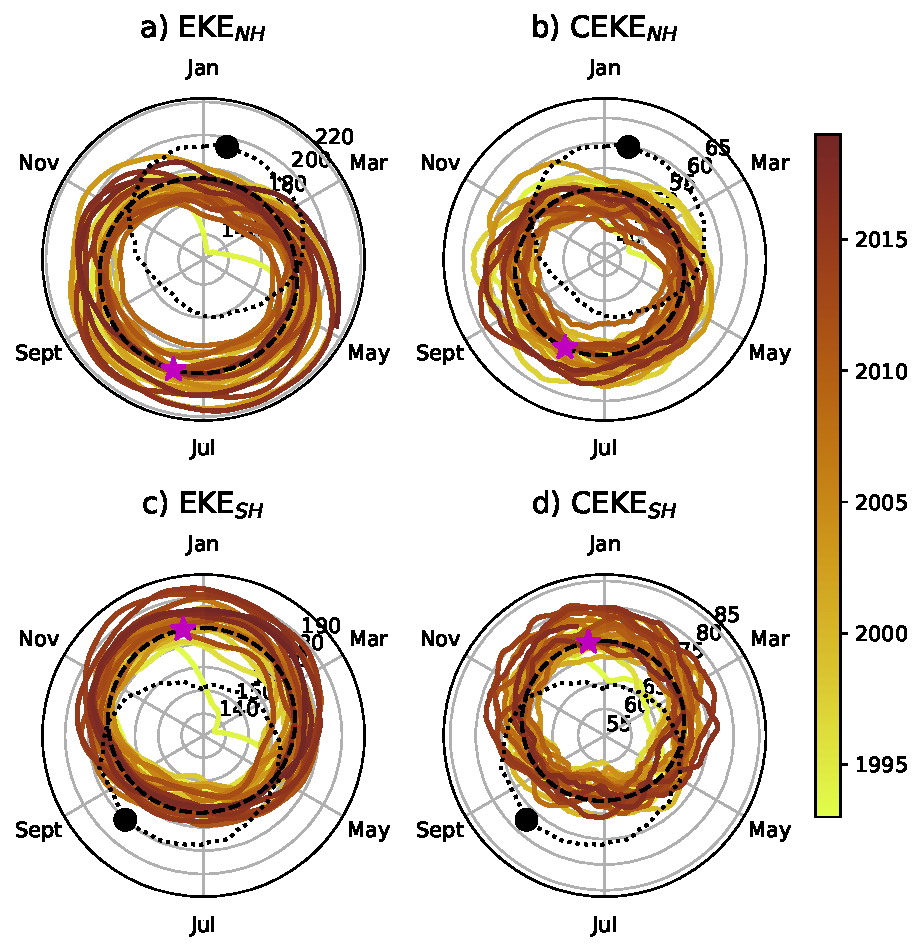
\includegraphics[width=95mm]{figures/All_polar_plots.pdf}
	    \caption{Hemispherical seasonality of eddy kinetic energy ($\EKE$), coherent eddy kinetic energy ($\CEKE$). 
		Panels a, and b show the northern hemisphere seasonal cycle, while panels c, and d correspond to the southern hemisphere. Dashed lines correspond to the seasonal cycle of the fields and dotted lines show the seasonal cycle of the wind magnitude smoothed over 120 days (moving average). 
		The green and magenta stars show the maximum of the seasonal cycle for the kinetic energy components and the wind magnitude, respectively. The line colors show the year.}
	    \label{fig:eddy_energy_polar}
	\end{figure}
	
	\section{Global Coherent Eddy Statistics}
	\label{subsec:CE_stats}

	% \textbf{Figure 5}
	% \begin{itemize}
		% \item A comparison with previous identified numbers show a consistent pattern in the eddy count. The difference in the magnitude could be a consequence of \citet{Chelton_Global_2007} filtering the coherent eddies with lifespans longer than 16 weeks. 
		% \item Both datasets show a large number of eddies in the East North Pacific, East North Atlantic, as well as the East South Pacific, East South Atlantic and East Indian Ocean. 
		% \item While the number of eddies detected in the tropics is quite small.
		% \item Furthermore, there are hotspots of numbers of eddies in other regions of the ocean, such as boundary currents and the Antarctic Circumpolar Current. 
		% \item An interesting feature shown in both datasets is a predominant patchiness where the count of the eddies is much larger. These puzzling pattern remains unknown. Although it looks like a propagation pattern, it could be that eddies persist for longer in those areas.
		% \item The eddy amplitude as expected is maximum at the boundary currents and hotspots in the southern ocean.
		% \item Interior of the gyres we can observe that there is and important amplitude of the coherent eddy field. 
		% \item Preferred eddy amplitude sign in boundary currents; positive amplitude polewards to the boundary current mean location, and negative amplitude equatorwards. This is consistent with the shed of coherent eddies from the boundary currents.
		% \item There regions with large $\CEKE$ ratio show also a large coherent eddy amplitude.
		% \item Absolute eddy amplitude has the similar signature as CEKE.
	% \end{itemize}

	Identified coherent eddies properties using automated algorithms allows to estimate the contribution and temporal changes in the number of eddies and the eddy amplitude. 
	Figure \ref{fig:eddy_stats_climatology} shows gridded global coherent eddy statistics; the number of eddies and eddy amplitude. 
	We checked M-M eddy count against \citet{Chelton_Global_2007} (Figure \ref{fig:eddy_stats_climatology}a-b). 
	Although the number of the identified eddies is larger in M-M, possibly due to the lifespan filter implemented by Chelton. 
	Overall both datasets reveal consistent spatial patterns, for example, both datasets show high abundance of eddies in the East North Pacific, East North Atlantic, as well as the East South Pacific, East South Atlantic and East Indian Ocean, and small number counts of eddies in the tropics and at high latitudes. An interesting pattern emerges in both eddy count datasets, where clusters with larger eddy counts are favored across the ocean, in addition to coherent eddy propagation patterns in boundary currents and regions in the Southern Ocean. Furthermore, these clusters of coherent eddies could be associated with topographic features, however it remains puzzling the consistency of the eddy count pattern.
	
	\begin{figure}
	    \centering
	    \includegraphics[width=1\textwidth]{figures/global_stats_V1.pdf}
	    \caption{Climatology of the coherent eddy statistics. a) Climatology of the number of coherent eddies ($\cEddy_n$) identified by \citet{Chelton_Global_2007};  b) Climatology of the number of coherent eddies ($\cEddy_n$) identified by \citet{Martinez_TKE_2019}; c) Climatology of the mean absolute coherent eddy amplitude ($\cEddy_{amp}$). d) Climatology of the mean coherent eddy amplitude ($\cEddy_{amp}$).}
	    \label{fig:eddy_stats_climatology}
	\end{figure}
	
	Regions with large counts of eddies have small absolute amplitudes (Figure \ref{fig:eddy_stats_climatology} c), while regions such as the boundary currents and Antarctic Circumpolar Current have the largest coherent eddy absolute amplitudes as shown by \citet{Chelton_The_2011}, followed by the interior of ocean gyres.
	Note that eddy amplitude highlights regions dominated by particular coherent eddy polarity, for example, boundary currents have a preferred sign (Figure \ref{fig:eddy_stats_climatology} d); positive amplitude polewards to the boundary current mean location, and negative amplitude equatorwards. 
	This sign preference is consistent with way coherent eddies are shed from boundary currents. 
	These global statistics reveal the absolute coherent eddy amplitude is a proxy of the $\CEKE$ with similar spatial patterns (Figure \ref{fig:eddy_climatology} \& Figure \ref{fig:eddy_stats_climatology} c) and showcases that regions where $\MCEKE$ has a large proportion of the $\MEKE$ (Figure \ref{fig:eddy_ratio}), the absolute coherent eddy amplitude is also large.

	

	\subsubsection{Seasonality}

	% \textbf{Figure 6}
	% \begin{itemize}
		% \item Seasonality of the number of eddies in the Northern Hemisphere peaks on May, while the Southern Hemisphere peaks on October. 
		% \item The seasonality of the amplitude of the eddies is consistent with those of the Coherent eddy kinetic energy. 
		% \item Interestingly, there is a 3 month lag to between the winds and the seasonality of the number of eddies, while the eddy amplitude responds approximately 6 months after the maximum winds. 
		% \item Note that both coherent eddy amplitudes seem to peak around the same time. 
		% \item If we look closely, the growing-shrinking concentric circles correspond to an increasing-decreasing trend. These are particularly obvious as a decrease in the eddy number in the Southern Hemisphere, and a increase in the eddy amplitude. 
	% \end{itemize}


	To further understand the seasonal cycle of $\CEKE$, we compute hemispherical seasonality of the coherent eddy properties (Figure \ref{fig:eddy_stats}). 
	The seasonality of the number of eddies in the Northern Hemisphere peaks on April (Figure \ref{fig:eddy_stats}a,c), while the Southern Hemisphere maximum number of eddies is around October (Figure \ref{fig:eddy_stats}e,g). 
	Meanwhile, the seasonality of the absolute eddy amplitude peaks in August and January for the Northern and Southern Hemispheres respectively (Figure \ref{fig:eddy_stats}b,d,f, and h). 
	As expected, the seasonality of the absolute eddy amplitude or intensity of the coherent eddies is consistent with the seasonal cycle of $\CEKE$. 
	Furthermore, a distinct lag of $\sim$3 months is observed between the forcing (winds) and eddy count, while the eddy amplitude maximum occurs $\sim$6 months after the seasonal maxima in winds. 
	This lag suggest the eddy number increases earlier in the year and through eddy-eddy interactions (merging of coherent eddies) the amplitude of the coherent eddy increases. This can be further explored by looking at the eddy diameter. Note that 90\% of identified eddies have diameters between 50 to 220 km (Figure \ref{fig:eddy_diameter}a), but more importantly, we observe in the Northern Hemisphere large-scale coherent eddies (diameter $>$ 120 km) maximum diameter occur during September, while small-scale coherent eddies (diameter $<$ 120 km) seasonal peak is during May (Figure \ref{fig:eddy_diameter}b). Meanwhile, in the Southern Hemisphere, the large-scale coherent eddies occurs in February, while the small-scale coherent eddies peak in December (Figure \ref{fig:eddy_diameter}c). This result is consistent with baroclinic instabilities generating many small coherent eddies early, which then are capable to merge and grow to become larger and more energetic. This process can be thought analogous to the inverse energy cascade, thus this mechanism not only drives the $\EKE$ seasonality, but also the seasonal cycle of coherent eddies. 

	Long-term changes can be observed in Figure \ref{fig:eddy_stats}a,b, e, and f where growing-shrinking concentric circles over time denote an increase-decrease trend of the field. 
	This is particularly evident in the Southern Hemisphere, where the number of eddies has decreased, the eddy amplitude has increased. 
	This result is consistent with the observed trends in $\EKE$ and mesoscale $\EKE$ in the Southern Ocean \citep{Hogg_Recent_2015,Martinez_Kinetic_2021}. 
	Furthermore, by analogy the long-term decrease in the number of coherent eddies and increase in coherent eddy amplitude could be a consequence of a long-term increase in the energy cascade, where interactions between eddies have generated a stronger coherent eddy field over the satellite record. 

	\begin{figure}
	    \centering
	    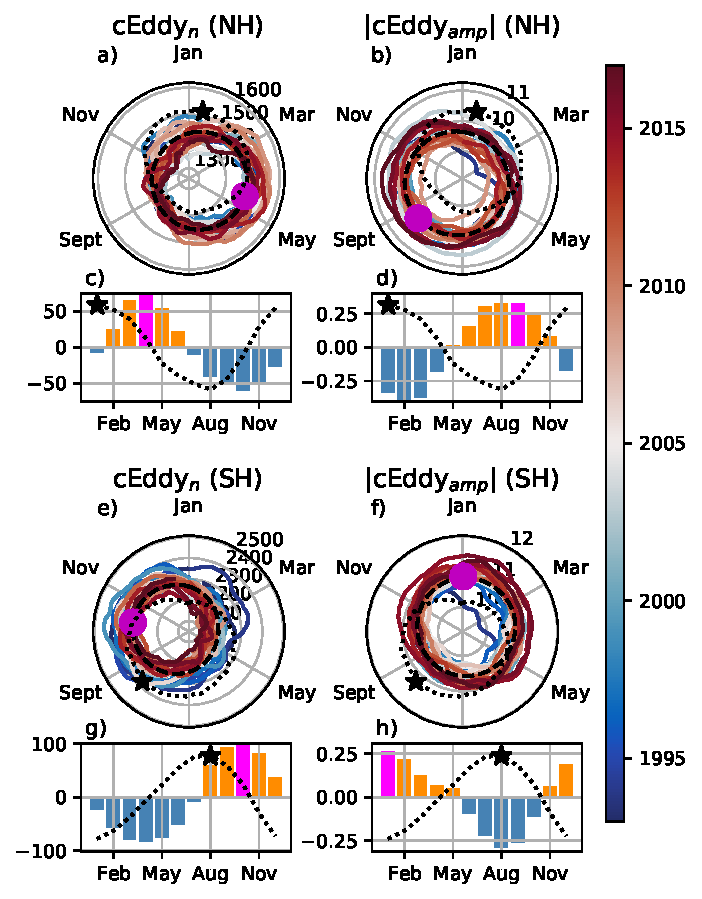
\includegraphics[width=95mm]{figures/All_polar_plots_eddy_stats_polarity_V3.pdf}
	    \caption{Hemispherical seasonality of the coherent eddy statistics;
		a,e) seasonal cycle of the number of coherent eddies ($\cEddy_n$); b,f) seasonal cycle of the mean coherent eddy amplitude ($\cEddy_{amp}$); c,g) seasonal cycle of the warm core coherent eddies amplitude (positive $\cEddy_{amp}$); d,h) seasonal cycle of the cold core coherent eddies amplitude (negative $\cEddy_{amp}$). Panels a,b and c show the northern hemisphere seasonal cycle, while panels d,e, and f correspond to the southern hemisphere. Dashed lines correspond to the seasonal cycle of the fields and dotted lines show the seasonal cycle of the wind magnitude smoothed over 120 days (moving average). The green and magenta stars show the maximum of the seasonal cycle for each field and the wind magnitude, respectively. The line colors show the year.}
	    \label{fig:eddy_stats}
	\end{figure}

	\begin{figure}
	    \centering
	    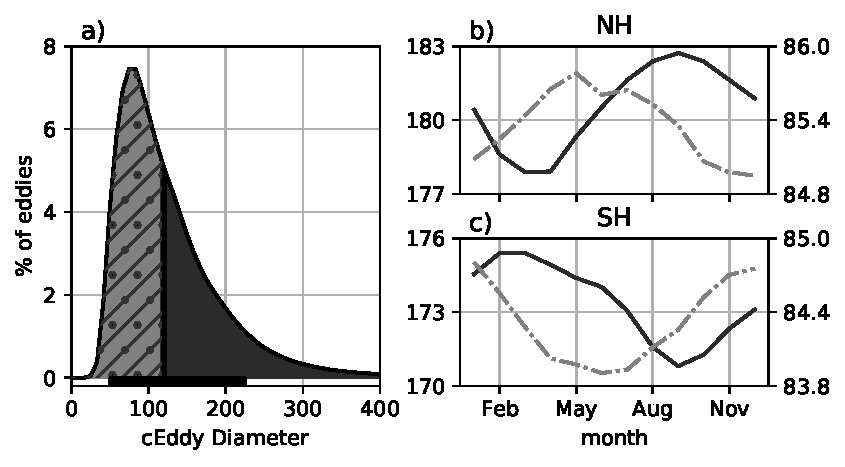
\includegraphics[width=95mm]{figures/eddy_diameter_seasonal.pdf}
	    \caption{Distribution of the identified eddy diameter and hemispherical seasonality of the coherent eddy diameter. a) Distribution in percentage of identified eddy amplitude, solid bar bellow distribution represents 90\% of the identified eddies. Seasonal cycle of the eddy diameter for the b) Northern Hemisphere and c) Southern Hemisphere. Dark solid line and area corresponds to coherent eddies with diameters larger than 120 km, while light gray dash-dotted line and area shows coherent eddies with diameters smaller than 120 km.}
	    \label{fig:eddy_diameter}
	\end{figure}

	The coherent eddy amplitude from positive coherent eddies and negative coherent eddies show similar seasonal cycles to the absolute eddy amplitude (Figure \ref{fig:eddy_stats_polar}). However, by separating the polarity contribution, its observed that the amplitude of negative coherent eddies in the Northern Hemisphere has decreased (Figure \ref{fig:eddy_stats_polar}b). In the Southern Ocean, the increase in absolute eddy amplitude is further corroborated as both coherent eddy polarities show an increase since the early 90s (Figure \ref{fig:eddy_stats_polar}e,f).


	% Should I add a seasonal cycle of the eddy radius? eddy area?, I've plotted it follows closely the eddy amplitude, which is expected, but as I just argued, the mean seasonal cycle shows on average a peak in summertime with diameters of 90 km, in fact, if I mask the radius with eddies larger than 90km, the seasonal cycle peaks in October, while eddies smaller than 90km peak on May. 

	\begin{figure}
	    \centering
	    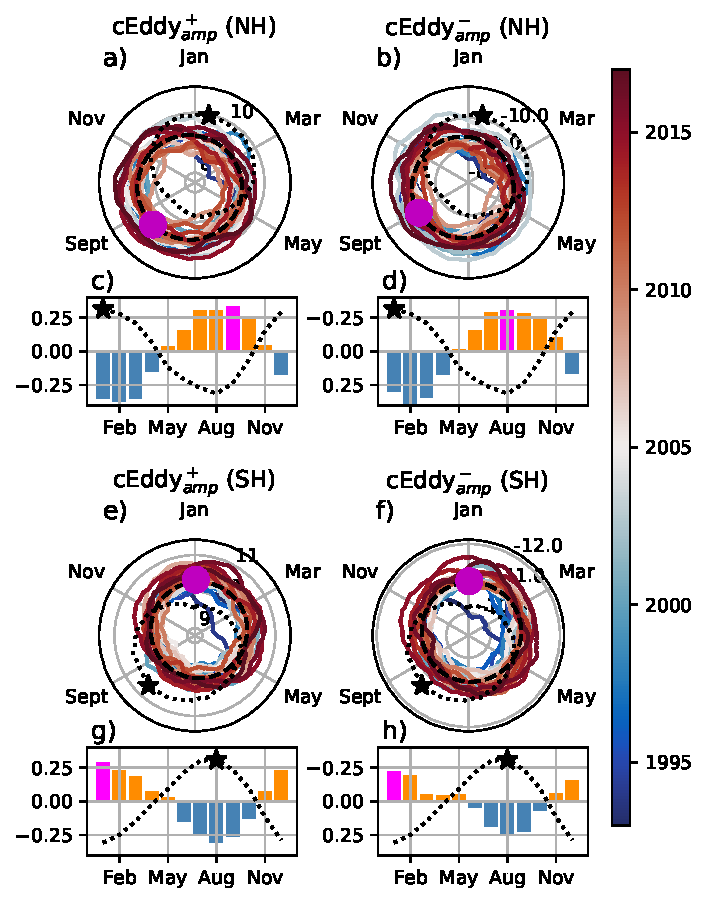
\includegraphics[width=95mm]{figures/All_polar_plots_eddy_stats_polarity_V4.pdf}
	    \caption{Hemispherical seasonality of the coherent eddy statistics;
		a,e) seasonal cycle of the number of coherent eddies ($\cEddy_n$); b,f) seasonal cycle of the mean coherent eddy amplitude ($\cEddy_{amp}$); c,g) seasonal cycle of the warm core coherent eddies amplitude (positive $\cEddy_{amp}$); d,h) seasonal cycle of the cold core coherent eddies amplitude (negative $\cEddy_{amp}$). Panels a,b and c show the northern hemisphere seasonal cycle, while panels d,e, and f correspond to the southern hemisphere. Dashed lines correspond to the seasonal cycle of the fields and dotted lines show the seasonal cycle of the wind magnitude smoothed over 120 days (moving average). The green and magenta stars show the maximum of the seasonal cycle for each field and the wind magnitude, respectively. The line colors show the year.}
	    \label{fig:eddy_stats_polar}
	\end{figure}

	\section{Trends}
	\label{sec:CE_trends}	
	
	% \textbf{Figure 13}
	% \begin{itemize}
		% \item The number and amplitude of coherent eddies from two eddy tracking algorithms show consistent trend patterns. 
		% \item In particularly, we observe a decrease in the number of eddies in the southern ocean, as well as sectors in the North Atlantic and North Pacific. 
		% \item Meanwhile the amplitude seems to be increasing in those same regions. 
		% \item Some of these regions have undergone a readjustment to stronger winds, thus the observed trends in the eddy amplitude suggests an intensification of the coherent eddy field to an increase in the forcing.
		% \item This increase is consistent with \citet{Martinez_Kinetic_2021}
	% \end{itemize}

	It is expected from the results presented in Figures \ref{fig:eddy_energy_polar}, \ref{fig:eddy_stats}, and  \ref{fig:eddy_stats_polar} a long-term readjustment of the coherent eddy field. 
	In particular, we now explore the long-term trends in the number of coherent eddies and absolute coherent eddy amplitude using both tracking algorithm datasets (Figure \ref{fig:eddy_stats_trends}). Both datasets show consistent trend and significance patterns. 
	Several regions in the ocean, such as the Southern Ocean, North Atlantic and North Pacific show a decrease in the number of eddies, meanwhile those same regions have a clear increase in the absolute coherent eddy amplitude. 
	This collocation of decrease in number and increase in eddy amplitude further supports an intensification of the coherent eddy field though eddy-eddy interactions. 
	These trends are similar to those observed in mesoscale eddy kinetic energy \citep{Martinez_Kinetic_2021} and provide additional evidence of a readjustment of the mesoscale eddy field over the last 3 decades.

	\begin{figure}
	    \centering
	    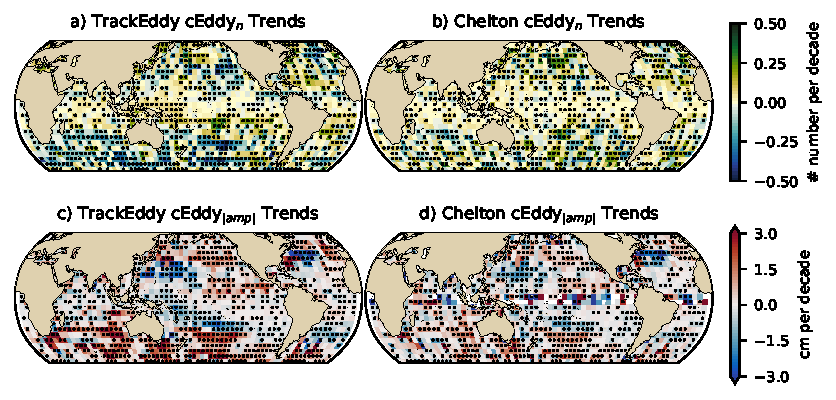
\includegraphics[width=1\textwidth]{figures/all_trackeddy_trends.pdf}
	    \caption{Trends of coherent eddy statistics. a) and b) Trends of the number of identified coherent eddies from satellite observations identified using TrackEddy, and those reported in Chelton's dataset. c) and e) Trends of the mean absolute value of identified coherent eddies amplitude from satellite observations identified using TrackEddy, and those reported in Chelton's dataset. Gray stippling shows regions that are statistically significant above the 95\% confidence level.
		}
	    \label{fig:eddy_stats_trends}
	\end{figure}


	\section{Regional}
	\label{sec:CE_regional_stats}
	
	For regions with relatively large proportions of $\CEKE$ (i.e., boundary currents and eastern currents), we investigate the seasonal and long-term variability in individual ocean regions.

	\subsection{Boundary Currents}
	
	The most energetic western boundary currents include; the Agulhas Current, the Kuroshio Current, and the Gulf Stream (Figures \ref{fig:Kuroshio}, \ref{fig:Gulf_Stream}, and \ref{fig:Agulhas}). In all these currents without exception and relative to the mean western boundary current location; (i) $\CEKE$ contains around 80\% of the $\EKE$ equatorward, (ii) the number of eddies is larger equatorward, and (iii) the absolute eddy amplitude is larger polewards of the mean western boundary current location. 
	
	a large amplitudes

	\textbf{Figure 10}
	\begin{itemize}
		\item Described similar to figure 7, 8, and 9
		\item Note that boundary currents have a consistent seasonal cycle in the positive and negative eddy amplitude.
		\item As expected, the seasonal cycle is opposite to BC in the northern hemisphere.
	\end{itemize}


	\textbf{Figure 11}
	\begin{itemize}
		\item Described similar to figure 7, 8, and 9
		\item Note that boundary currents have a consistent seasonal cycle in the positive and negative eddy amplitude.
	\end{itemize}

	\begin{figure}
	    \centering
	    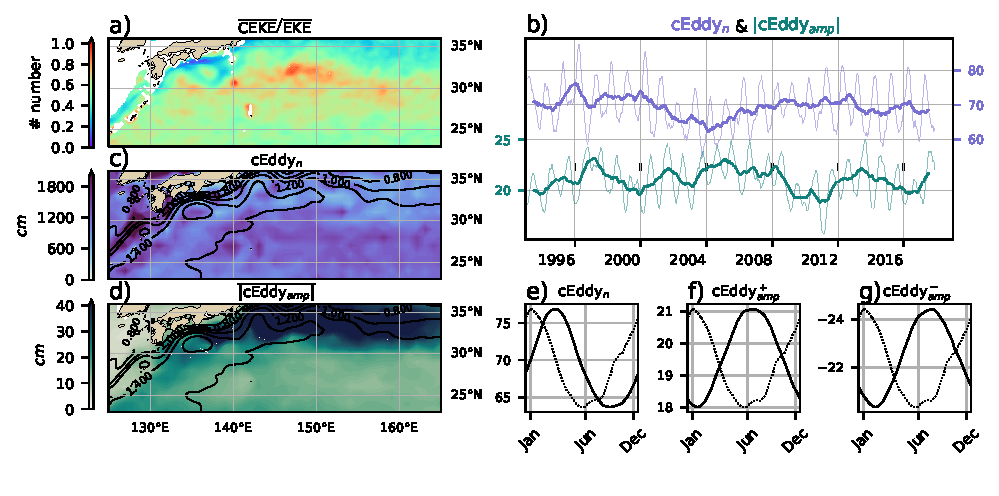
\includegraphics[width=1\textwidth]{figures/regional_ratios_and_stats_V3_4.pdf}
	    \caption{Same as Figure \ref{fig:leeuwin_cycle} but for the Kuroshio Current.}
	    \label{fig:Kuroshio}
	\end{figure}

	\textbf{Figure 12}
	\begin{itemize}
		\item Described similar to figure 7, 8, and 9
		\item Note that boundary currents have a consistent seasonal cycle in the positive and negative eddy amplitude.
		\item \textcolor{purple}{Delete Fig 11 or 12, they are really similar. What do you think?}
	\end{itemize}

	\begin{figure}
	    \centering
	    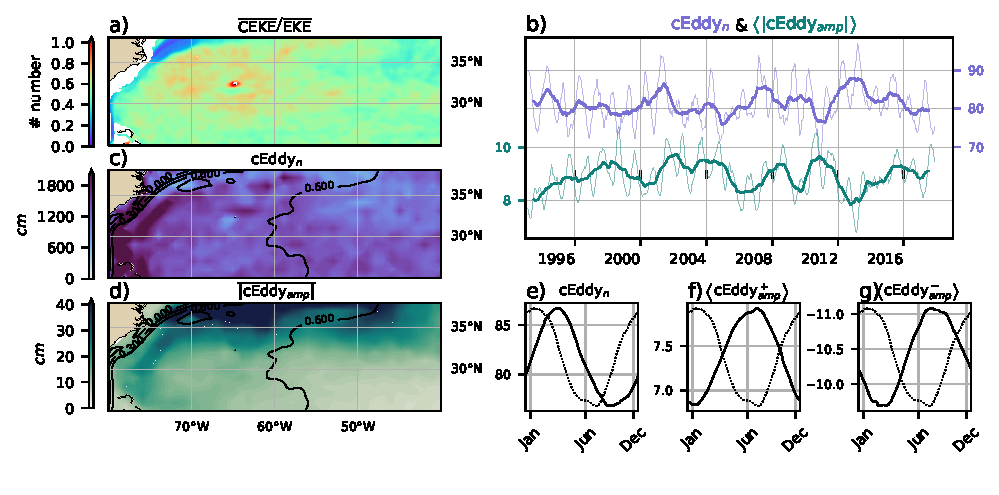
\includegraphics[width=1\textwidth]{figures/regional_ratios_and_stats_V3_5.pdf}
	    \caption{\textbf{Move to supplementary} Same as Figure \ref{fig:leeuwin_cycle} but for the Gulf Stream.}
	    \label{fig:Gulf_Stream}
	\end{figure}


	\begin{figure}
	    \centering
	    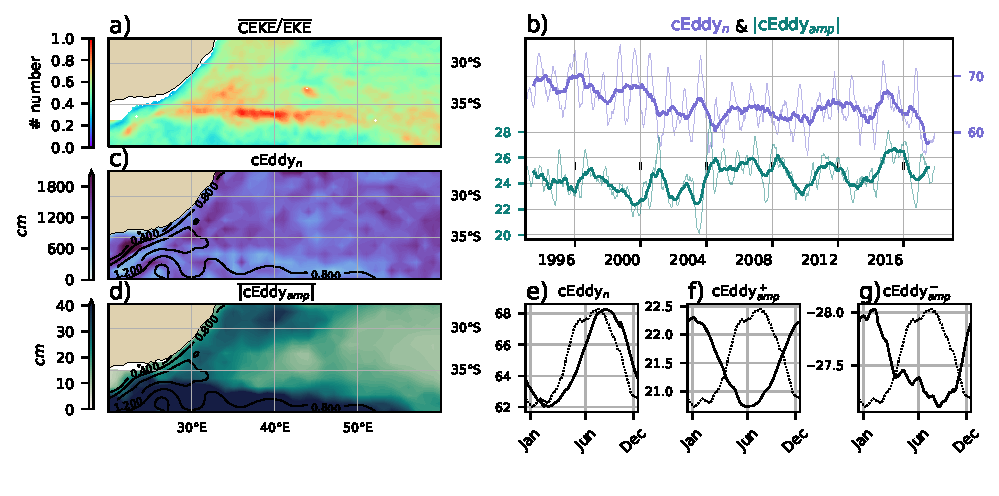
\includegraphics[width=1\textwidth]{figures/regional_ratios_and_stats_V3_2.pdf}
	    \caption{Same as Figure \ref{fig:leeuwin_cycle} but for the Agulhas Current.}
	    \label{fig:Agulhas}
	\end{figure}

	\subsection{Eastern currents}


	\textbf{Figure 7}
	\begin{itemize}
		\item South of the Leeuwin Current there is an important dominance fo the coherent eddy field, where it explains around 80\% of the eddy kinetic energy.
		\item Although this region does not have a large $\EKE$, we can observe a considerable amount of eddies across the region, but more importantly the coherent eddy amplitude is particularly large in those regions with coherent eddy dominance. 
		\item The solid lines show an decrease in the number of eddies, but an increase in the eddy amplitude. 
		\item Moreover, the coherent eddy number peaks in August.
		\item Meanwhile coherent eddies with the positive amplitude have a smaller amplitude than the negative, furthermore, the positive eddies peak in Jun and show a interannual modulation, while the negative eddies peak in October. 
		\item Research regional dynamics (Add here why we may expect this response.)
	\end{itemize}

	\begin{figure}
	    \centering
	    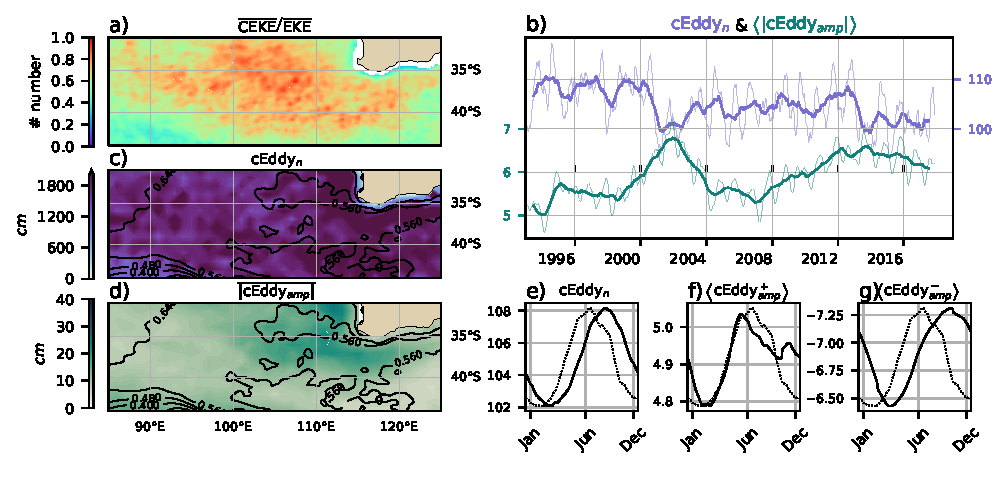
\includegraphics[width=1\textwidth]{figures/regional_ratios_and_stats_V3_0.pdf}
	    \caption{ Climatology of the eddy field and coherent eddy field at the Leeuwin Current. a) Ratio of mean coherent eddy kinetic energy ($\MCEKE$) versus mean eddy kinetic energy ($\MEKE$); b) Thick lines show the running average over 2 years and thin lines show the running average over 90 days of the coherent eddy number sum and the average absolute coherent eddy amplitude; c) Map of the number of eddies; d) Map of the average absolute coherent eddy amplitude; e) Seasonal cycle of the number of eddies f) Seasonal cycle of the positive coherent eddy amplitude. g) Seasonal cycle of the negative coherent eddy amplitude.}
	    \label{fig:leeuwin_cycle}
	\end{figure}

	% \textbf{Figure 8}
	% \begin{itemize}
	% 	\item South west of the Hawai'i there is an important influence of the coherent eddies.
	% 	\item Although, near we observe a large amount of numbers of eddies in both eddy count form Chelton and JMM, the amplitude is again responsible of the coherent eddy dominance. 
	% 	\item Note the eddy number peaks in March, while the positive eddy amplitude peaks in October, while the negative eddies peak in June.
	% 	\item Research regional dynamics (Add here why we may expect this response.)
	% \end{itemize}

	% \begin{figure}
	%     \centering
	%     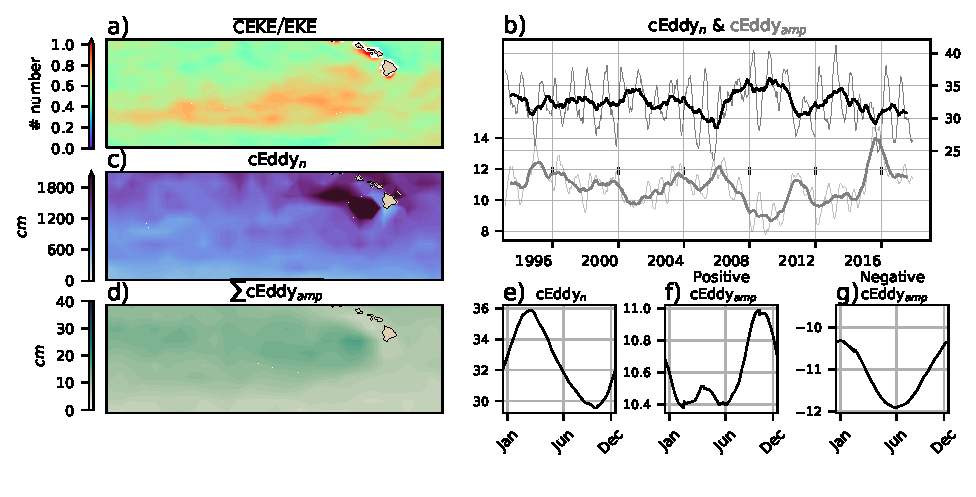
\includegraphics[width=1\textwidth]{figures/regional_ratios_and_stats_V3_1.pdf}
	%     \caption{Same as Figure \ref{fig:leeuwin_cycle} but for the Central North Pacific.}
	%     \label{fig:east_tropical_cycle}
	% \end{figure}

	\textbf{Figure 9}
	\begin{itemize}
		\item Here we observe that the number of eddies and eddy amplitude are large in the area where the coherent eddies dominate the eddy field.
		\item Dynamically, in this region eddies are generated due to Rossby wave propagation along the coast that becomes unstable and sheds eddies at the Tehuantepec Gulf.
		\item The seasonal cycle shows a peak in Jun, while the positive amplitude is observed in March and the negative amplitude maximum occurs in September. 
		\item Research regional dynamics (Add here why we may expect this response.)
	\end{itemize}

	\begin{figure}
	    \centering
	    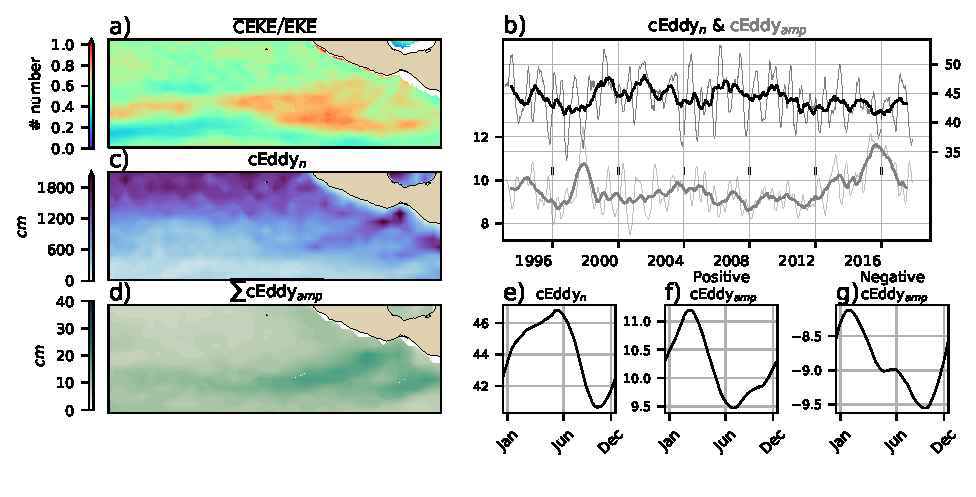
\includegraphics[width=1\textwidth]{figures/regional_ratios_and_stats_V3_3.pdf}
	    \caption{Same as Figure \ref{fig:leeuwin_cycle} but for the East Tropical Pacific.}
	    \label{fig:south_atlantic_cycle}
	\end{figure}
	
	\section{Summary and Conclusions}	
	\label{sec:Conclusions}
	
	\acknowledgments
	\citet{Chelton_mesoscale_2013} dataset was produced by SSALTO/DUACS and distributed by AVISO+ (\url{https://www.aviso.altimetry.fr/}) with support from CNES, developed and validated in collaboration with E.Mason at IMEDEA.
	Global coherent eddy reconstruction, coherent and non-conherent eddy kinetic energy datasets, in addition to gridded coherent eddy tracking datasets are publicly available at (\url{https://doi.org/10.5281/zenodo.4646429}). 
	All analyses and figures in this manuscript are reproducible via Jupyter notebooks and instructions can be found in the Github repository \texttt{CEKE\_climatology} (\url{https://github.com/josuemtzmo/CEKE_climatology}). Trends used the Python Package xarrayMannKendall (\url{https://doi.org/10.5281/zenodo.4458776})
	
	\bibliography{biblio.bib}
	
\end{document}
